    \subsection{Triển khai Hệ thống Gợi ý}
\label{subsec:recsys_implementation}

Hệ thống VieVu triển khai hai cơ chế gợi ý chính để đề xuất địa điểm cho người dùng. Mục này sẽ trình bày chi tiết việc triển khai kỹ thuật cho cơ chế gợi ý địa điểm liên quan dựa trên nội dung (Content-Based Filtering). Việc triển khai hệ thống gợi ý chính dựa trên Neural Network sẽ được đề cập ở phần sau (hoặc trong một mục riêng).

\subsubsection{Gợi ý Địa điểm Liên quan (Content-Based)}
\label{subsubsec:cb_recsys_impl}
Hệ thống gợi ý địa điểm liên quan này hoạt động bằng cách kết hợp điểm đánh giá chất lượng/phổ biến nội tại của địa điểm với độ tương đồng về mặt nội dung văn bản, được triển khai qua các bước sau:

\begin{enumerate}
 

\item  \textbf{Tính toán Điểm Nội tại ($Score_{Item}$)}
Trước tiên, hệ thống tính toán một điểm số đại diện cho chất lượng và độ phổ biến của mỗi điểm tham quan (\texttt{attractions}). Điểm này dựa trên điểm đánh giá trung bình có trọng số ($Score_{WeightedAvg}$) được làm mượt để giảm thiểu ảnh hưởng của số lượng đánh giá ít, tính theo công thức:
$$Score_{WeightedAvg} = \frac{R \times v + C \times m}{v + m}$$
trong đó $R$ là điểm trung bình gốc, $v$ là số lượt đánh giá của địa điểm, $C$ là điểm trung bình của tất cả địa điểm, và $m$ là ngưỡng số lượt đánh giá tối thiểu cần thiết. Sau đó, giá trị $Score_{WeightedAvg}$ và điểm \texttt{hot\_score} của địa điểm được chuẩn hóa về thang [0, 1] ($ScaledWeightedAvg$, $ScaledHotScore$) và kết hợp thành điểm nội tại cuối cùng $Score_{Item}$ với các trọng số $w_{hs}$ và $w_{wa}$ (ví dụ: $w_{hs}=0.6, w_{wa}=0.4$):
$$Score_{Item} = w_{hs} \times ScaledHotScore + w_{wa} \times ScaledWeightedAvg$$
% (Tham khảo mã nguồn tính điểm tại Đoạn mã \ref{lst:score_calculation}) % <<< Placeholder

\item  \textbf{Biểu diễn Nội dung và Tính Độ tương đồng Cosine}
Nội dung văn bản của các địa điểm (tên, mô tả, địa chỉ, loại hình,v.v.) được tiền xử lý và tổng hợp thành một trường \texttt{bag\_of\_words}. Trường này sau đó được vector hóa bằng kỹ thuật TF-IDF (sử dụng \texttt{TfidfVectorizer} từ Scikit-learn \cite{sklearn_lib}, có loại bỏ từ dừng tiếng Việt) để tạo ra ma trận vector \texttt{tfidf\_matrix}. Độ tương đồng về nội dung giữa hai địa điểm bất kỳ (biểu diễn bởi vector $\vec{a}$ và $\vec{b}$) được đo bằng Cosine Similarity.
Kết quả là ma trận độ tương đồng \texttt{cos\_sim} giữa tất cả các cặp địa điểm.
% (Tham khảo mã nguồn xử lý text và TF-IDF tại Đoạn mã \ref{lst:tfidf_cosine_code}) % <<< Placeholder

    \item  \textbf{Hàm Gợi ý và Kết hợp Điểm}
Hàm gợi ý \texttt{get\_related\_attractions} nhận ID của một địa điểm đang xem làm đầu vào. Hàm này lấy điểm nội tại $Score_{Item}$ và các giá trị độ tương đồng nội dung ($Similarity$) của địa điểm đó với các địa điểm khác từ ma trận \texttt{cos\_sim}. Một điểm số gợi ý cuối cùng ($Score_{Final}$) cho mỗi địa điểm tiềm năng được tính bằng cách kết hợp hai loại điểm trên với trọng số $w_{sim}$ (ví dụ: $w_{sim}=0.7$):
$$Score_{Final} = w_{sim} \times Similarity + (1 - w_{sim}) \times Score_{Item}$$
Cuối cùng, hàm trả về Top N địa điểm có $Score_{Final}$ cao nhất (không bao gồm địa điểm đầu vào) thông qua API endpoint của FastAPI.
\end{enumerate}

\subsubsection{Gợi ý Địa điểm Chính (Neural Network - Hybrid)}
\label{subsubsec:nn_recsys_impl_final} % Label mới

Hệ thống gợi ý chính của VieVu, nhằm mục đích đề xuất các địa điểm phù hợp nhất với sở thích cá nhân của từng người dùng, được xây dựng dựa trên mô hình Neural Network (NN) theo cách tiếp cận Hybrid.
\begin{enumerate}
    \item \textbf{Mục tiêu và Cách tiếp cận Hybrid}
    
Mô hình này được thiết kế để dự đoán mức độ phù hợp (thể hiện qua điểm rating dự đoán) giữa một người dùng và một địa điểm cụ thể. Gọi là Hybrid vì nó sử dụng kết hợp ba nguồn thông tin: (1) Đặc trưng người dùng (User Features), bao gồm các thông tin về sở thích đối với các loại hình du lịch khác nhau, có thể được thu thập từ khảo sát ban đầu hoặc suy ra từ hành vi; (2) Đặc trưng địa điểm (Item Features), bao gồm các thuộc tính số như độ "hot", giá cả, điểm đánh giá trung bình và biểu diễn One-Hot Encoding của 88 loại hình du lịch mà địa điểm đó thuộc về; (3) Dữ liệu đánh giá (Ratings) làm tín hiệu hướng dẫn quá trình học. Mô hình được xây dựng và huấn luyện bằng thư viện TensorFlow cùng với Keras API \cite{tensorflow_lib, keras_lib}.
    
    \item \textbf{Chuẩn bị Dữ liệu Đặc trưng và Tạo Dữ liệu Rating Giả lập}

Quá trình chuẩn bị dữ liệu bao gồm các bước:
    \begin{itemize}
        \item Tải dữ liệu cho 3500 người dùng từ tệp \texttt{user\_preferences\_with\_price.csv} và cho 1006 địa điểm từ tệp \texttt{attraction\_unique\_vectors.csv}. Điểm đánh giá trung bình (\texttt{avg\_rating}) của địa điểm trong file vector đã được tính toán lại bằng công thức làm mượt để giảm sai lệch do số lượng đánh giá ít.
        \item Tạo dữ liệu Rating giả lập: Do hạn chế về dữ liệu rating thực tế, bộ dữ liệu huấn luyện chính (lưu trong \texttt{user\_ratings\_data\_updated.csv}) được tạo ra bằng phương pháp giả lập. Dựa trên \texttt{avg\_rating} và \texttt{rating\_count} thống kê gốc của mỗi địa điểm, hệ thống thực hiện gán ngẫu nhiên các điểm rating cho các cặp (user\_id, attraction\_id) sao cho phân phối rating tổng hợp của từng địa điểm trong bộ dữ liệu giả lập này tương đồng với thống kê gốc.
        \item Kết hợp (merge) dữ liệu đặc trưng người dùng, đặc trưng địa điểm và rating giả lập để tạo thành tập dữ liệu huấn luyện cuối cùng, trong đó mỗi mẫu bao gồm cặp vector đặc trưng (user, item) và một điểm rating giả lập làm nhãn (target).
        \item Chia tập dữ liệu thành tập huấn luyện (90\%) và tập kiểm thử (10\%).
    \end{itemize}
    
    \item \textbf{Kiến trúc Mô hình Neural Network }

Mô hình NN được thiết kế theo kiến trúc hai nhánh song song để học biểu diễn riêng cho người dùng và địa điểm trước khi kết hợp:

\begin{itemize}
    \item \textbf{Nhánh Người dùng:} Nhận đầu vào là vector đặc trưng người dùng. Dữ liệu đi qua các lớp mạng nơ-ron kết nối đầy đủ (Dense) với hàm kích hoạt ReLU (2 lớp, Dense(128) -> Dense(64)).
    \item \textbf{Nhánh Địa điểm:} Nhận đầu vào là vector đặc trưng địa điểm. Dữ liệu cũng đi qua các lớp Dense tương tự (Dense(128) -> Dense(64)).
    \item \textbf{Kết hợp và Dự đoán:} Output từ hai nhánh được ghép nối (Concatenate). Vector kết hợp này tiếp tục đi qua một lớp Dense (Dense(64)) và cuối cùng là một lớp Dense với 1 nơ-ron và hàm kích hoạt tuyến tính ('linear') để đưa ra dự đoán rating cuối cùng.
\end{itemize}

\lstset{language=python}
\begin{lstlisting}[
    caption=Thiết lập mô hình Neural Network,
    label=lst:nn_model,
    captionpos=t,
    belowcaptionskip=10pt,
    basicstyle=\small\ttfamily,
    breaklines=true,
    showstringspaces=false,
    inputencoding=utf8] 
    user_layer = Dense(128, activation='relu')(input_user)
    user_layer = Dense(64, activation='relu')(user_layer)
    attraction_layer = Dense(128, activation='relu')(input_attraction)
    attraction_layer = Dense(64, activation='relu')(attraction_layer)
    merged = Concatenate()([user_layer, attraction_layer])
    merged = Dense(64, activation='relu')(merged)
    output = Dense(1, activation='linear')(merged)
    model = Model(inputs=[input_user, input_attraction], outputs=output)
    model.compile(optimizer=Adam(learning_rate=0.001), loss='mse', metrics=['mae'])
    model.summary()

\end{lstlisting}
    % (Sơ đồ kiến trúc mô hình có thể xem tại Hình~\ref{fig:nn_arch}) % <<< Placeholder
    
    \item \textbf{Quá trình Huấn luyện Mô hình}
   
Mô hình được huấn luyện với mục tiêu tối thiểu hóa sai số giữa rating dự đoán và rating giả lập trong tập huấn luyện.
    \begin{itemize}
        \item \textbf{Hàm mất mát (Loss Function):} Mean Squared Error (MSE) được sử dụng.
        \item \textbf{Thuật toán tối ưu (Optimizer):} Adam với learning rate 0.001.
        \item \textbf{Độ đo đánh giá (Metrics):} Mean Absolute Error (MAE) được theo dõi trong quá trình huấn luyện và đánh giá trên tập kiểm thử.
        \item \textbf{Quá trình huấn luyện:} Mô hình được huấn luyện trong 30 epochs với batch size là 32.
        \item \textbf{Lưu trữ mô hình:} Mô hình có kết quả tốt nhất trên tập kiểm thử được lưu lại vào tệp (\texttt{model\_unique\_128}) để có thể tải lại và sử dụng cho việc gợi ý mà không cần huấn luyện lại từ đầu.
    \end{itemize}

    \begin{figure}[H]
        \centering
        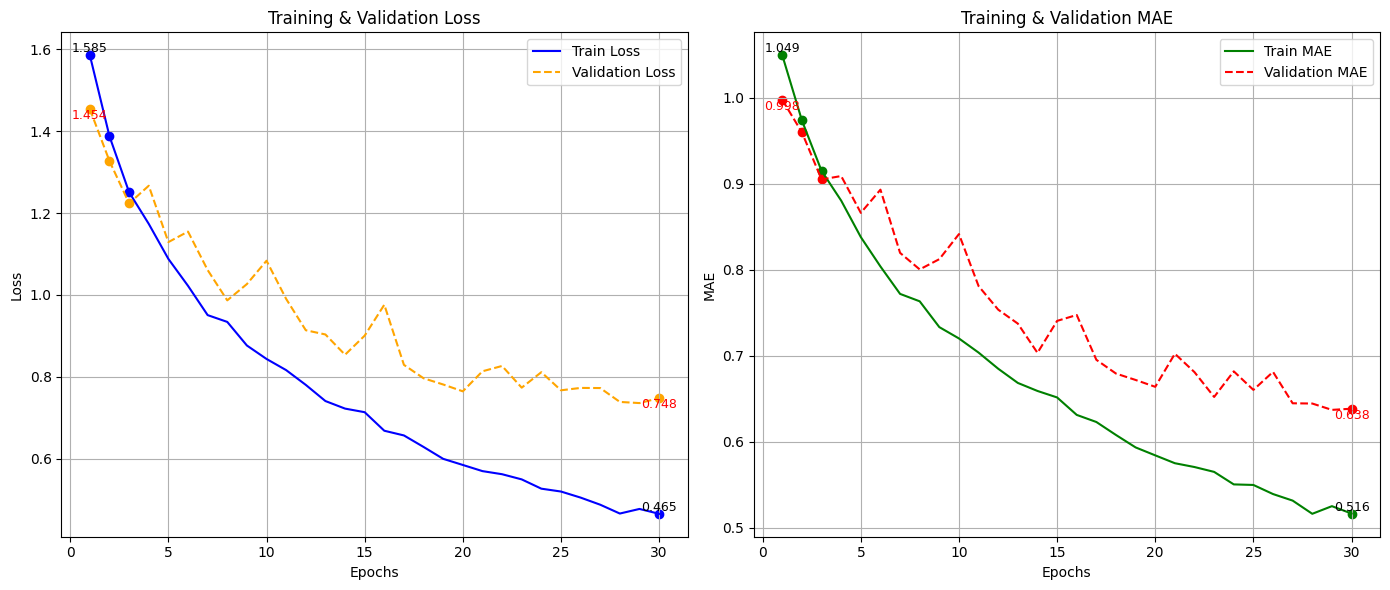
\includegraphics[width=1\textwidth]{figures/c4/128.png}
        \caption{Hiệu suất mô hình qua độ đo MAE.}
        \label{fig:mae}
    \end{figure}
    \noindent Quá trình huấn luyện được thực hiện trong 30 epochs với các cấu hình như trên. Kết quả huấn luyện được trực quan hóa trong Hình~\ref{fig:mae}  cho thấy cả giá trị hàm mất mát (Loss) và sai số tuyệt đối trung bình (MAE) trên tập huấn luyện (training set) và tập kiểm chứng (validation set) đều giảm đáng kể, chứng tỏ mô hình đã có khả năng học được các mẫu từ dữ liệu. Mô hình cuối cùng đạt được MAE khoảng 0.64 trên tập kiểm chứng, cho thấy sai số dự đoán trung bình chấp nhận được, mặc dù biểu đồ cũng thể hiện có một khoảng cách nhất định giữa hiệu năng trên tập huấn luyện và tập kiểm chứng, là dấu hiệu của overfitting. Mô hình với trọng số tốt nhất đã được lưu lại để sẵn sàng cho bước triển khai gợi ý.

\end{enumerate}
Như vậy, việc triển khai hệ thống gợi ý địa điểm chính của VieVu đã hoàn thành thông qua việc xây dựng và huấn luyện mô hình Neural Network Hybrid theo kiến trúc two-tower. Bằng cách kết hợp thông tin đặc trưng chi tiết của người dùng và địa điểm cùng với tín hiệu học hỏi từ dữ liệu rating (dù được tạo giả lập), mô hình đã được tối ưu hóa để dự đoán mức độ phù hợp. Hệ thống gợi ý cuối cùng được tích hợp vào API server, sẵn sàng cung cấp các đề xuất địa điểm được cá nhân hóa, góp phần nâng cao khả năng khám phá và trải nghiệm người dùng trong ứng dụng.